\documentclass[xcolor=svgnames]{beamer}
\usepackage{graphics}
\usepackage{amsmath}
\usepackage[english]{babel}
\usetheme{Warsaw}
\useinnertheme{rounded}
\usefonttheme{serif}
\setbeamertemplate{navigation symbols}{}
\begin{document}
\title{M311 Calculus III Recitation}
	\author{Tim Lai }
	\institute{Indiana University}
%	\titlegraphic{\includegraphics[width=5cm]{Logo.jpg}}
	\date{Fall 2019}
\frame{\titlepage}
\begin{frame}
\frametitle{Projections}
\framesubtitle{Section 12.1}
\begin{center}
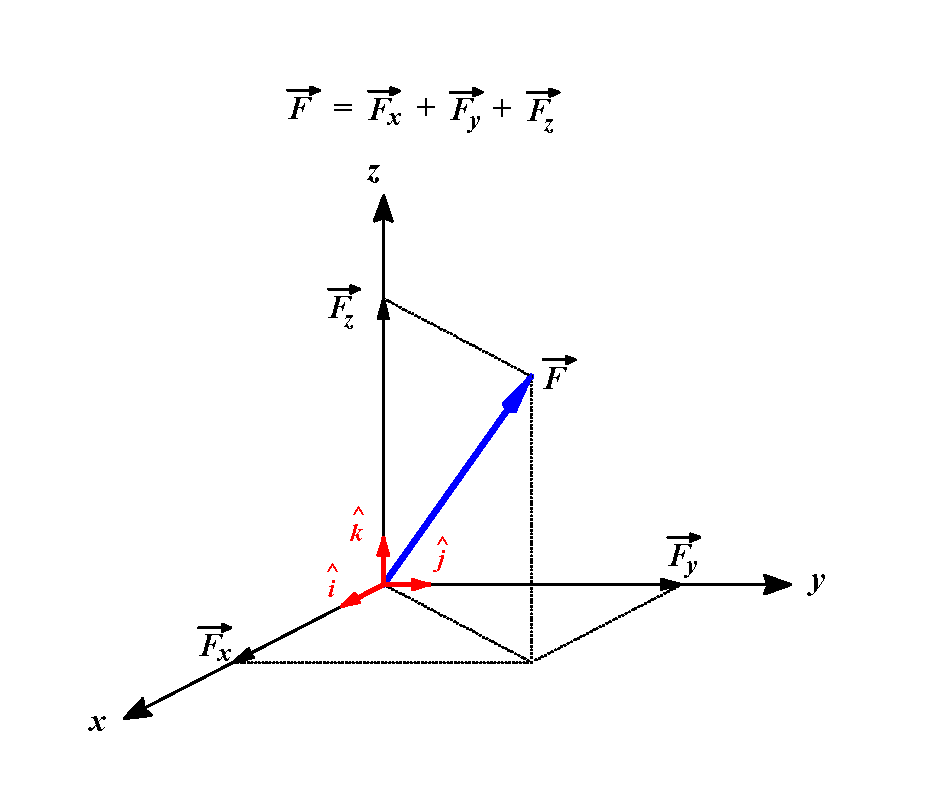
\includegraphics[width=8cm]{3D_vector_component.png}
\end{center}
\end{frame}
\begin{frame}
\frametitle{Vector Operations}
\framesubtitle{Section 12.2}
Suppose $a = \langle 2,3,0 \rangle$ and $b = \langle -1, 0,1 \rangle$. 
Then
\begin{align*}
 |a + 2b| &= |  \langle 2,3,0 \rangle + 2  \langle -1, 0,1 \rangle | \\
&= | \langle 2,3,0 \rangle +\langle -2, 0,2 \rangle | \\
& = | \langle 0,3,2 \rangle | \\
&= \sqrt{0^2 + 3^2 + 2^2} \\
&= \sqrt{13}
\end{align*}
\end{frame}
\begin{frame}
\frametitle{Dot Product}
\framesubtitle{Section 12.3}
Dot products are a special case of matrix multiplication.

Suppose $a = \langle 2,3,0 \rangle$ and $b = \langle -1, 0,1 \rangle$. Then
\[
 a \cdot b = 2(-1) + 3(0) + 0(1) = -2
\]
Compare to $(2,3,0) (-1,0,1)^T$ where these are now thought of as matrices and $T$ denotes transpose. 
\end{frame}
\begin{frame}
\frametitle{Dot Product}
\framesubtitle{Important properties and uses}
\begin{itemize}
	\item Dot product gives a computationally conducive way to get a handle on angles between vectors. 
	\item $a \cdot b = |a||b| \cos \theta$ where $\theta$ is the angle between the two vectors. 
	\item In particular, since $\cos \theta = 0$ if and only if $\theta = \pi / 2 + k \pi$, we can conclude that $a \perp b \Leftrightarrow a \cdot b = 0$. 
	\item Note: dot product takes two vectors and gives a number. 
	\item In the previous example, since the dot product was nonzero, we can conclusively say that the vectors were not orthogonal. 
\end{itemize}
\end{frame}
\begin{frame}
\frametitle{Cross Product}
\framesubtitle{Problem 20}
Computing unit vectors perpendicular to $j - k$ and $i + j$:
\[
	(j-k) \times (i + j) = i - j - k
\]
However, this vector is not a unit vector! We must normalize by dividing by the magnitude, in this case, $1/\sqrt{3}$. 
\end{frame}
\begin{frame}
\frametitle{Cross Product}
\framesubtitle{Problem 27}
Finding the area of a parallelogram given the corner points. 
\begin{enumerate}
\item Plot the vectors and draw in the parallelogram
\item Identify two vectors that determine the parallelogram
\item Compute the magnitude of the cross product. 
\end{enumerate}
\end{frame}
\begin{frame}
\frametitle{Cross Product}
\framesubtitle{Problem 29}
Finding a vector orthogonal to the plane given three points on the plane. 
\begin{enumerate}
\item The plane through $P,Q,R$ must contain the vectors formed by the points, such as $PQ$ and $PR$. 
\item Find a vector orthogonal to both of these vectors with the corss product.
\item This vector must then be orthogonal to the plane itself. 
\end{enumerate}
\end{frame}
\begin{frame}
\frametitle{Lines and Planes}
\framesubtitle{Problem 10}
Find equation of line containing $P_0 = (2,1,0)$ and direction perpendicular to $i+j$ and $j + k$. 
\begin{enumerate}
\item Compute a vector orthogonal to both 
\item Say the vector is $(a,b,c)$. Then the parametric equation is $x = 2 + at, y = 1 + bt, z = ct$. 
\end{enumerate}
\end{frame}
\begin{frame}
\frametitle{Lines and Planes}
\framesubtitle{Problem 17}
Line segment from $r_0 = \langle 6,-1,9 \rangle$ to $r_1 = \langle 7,6,0 \rangle $:
\begin{align*}
r(t) &= (1-t)r_0 + tr_1 \\
&= (1-t)\langle 6, -1, 9 \rangle  + t \langle 7, 6, 0 \rangle \\
&= \langle 6, -1, 9 \rangle - t\langle 6, -1, 9 \rangle + t \langle 7, 6 , 0 \rangle \\
&= \langle 6, -1, 9 \rangle + t \langle 1, 7, -9 \rangle
\end{align*}
\end{frame}
\begin{frame}
\frametitle{Lines and Planes}
\framesubtitle{Parallel (Problem 20)}
How do you determine whether two lines are parallel given their direction vectors? 
\begin{enumerate}
\item Say we have two lines with direction vectors $v_1$ and $v_2$. 
\item Determine whether there exists a constant such that $v_1 = c v_2$. 
\item If there is, then the two lines are parallel. If not, it may be possible that the lines intersect or are skew. 
\end{enumerate}


\end{frame}
\begin{frame}
\frametitle{Lines and Planes}
\framesubtitle{Finding equations of planes}
\begin{itemize}
	\item The equation of a plane depends heavily on the normal vector.
	\item Main goal: find the normal vector
	\item Our strategy to doing so involves taking two cross products of vectors.
	\item Therefore, in all problems, get such vectors, either on the plane, parallel to the plane, etc.
\end{itemize}
\end{frame}

\begin{frame}
\frametitle{Vector Functions}
\framesubtitle{Problems 12, 21, and 27}
\begin{itemize}
\item Note that both problems have one coordinate equal to $\cos t$ and another coordinate has $\sin t$. 
\item Use $\sin^2 t + \cos ^2 t = 1$ 
\item Incorporate the third coordinate
\end{itemize}
\end{frame}
\end{document}